\section{实验}
\label{sec:exp}
\textbf{实验设置。} 每次运行都是在线阶段的一次完整预演：在课程发布的仿真器的本地副本（sha256 固定）上，从训练行出发顺序进行
20 次调用、每次 50 个点。我们比较 \emph{v1}（固定类别份额的分块下降）、\emph{v2}（v1 加上由训练行得出的偏移偏置）、\emph{v4}
（v2 加上证据驱动的分配）以及消融变体 \emph{v4j}（j 表示联合），即去掉分块结构的 v4：每个候选从当前最好点或一个实测精英点（本次运行中
$R$ 最低的点之一）出发同时改动三栋建筑（每栋各自做一次同类移动），没有基点和组合点，平台过滤和改进坐标的重新施加也关闭，
因为两者都需要单块结果；代理模型、移动类别、信任尺度和后验份额都不变。一个后期减少代理模型挑选的变体（v3）在一次运行
（107.78）后被放弃。指标是 20 次调用后的最佳 $R$。不同策略消耗随机数流的方式不同，因此种子在策略之间不配对，只有一个例外：
提交的策略 h7 在第 1--11 次调用中与 v4 相同，在它的三个种子上可以与 v4 配对。我们报告种子上的均值 $\pm$ 标准差，以及对
均值之差的精确双侧置换检验。

\begin{table}[t]
\centering
\caption{真实仿真器上 20 次调用 $\times$ 50 个点之后的最佳 $R$（kWh）。第10次：第 10 次调用后的平均最佳 $R$。$p$：与 v4 比较的精确置换检验。v4j 还去掉了平台过滤和坐标重新施加。参考：最佳训练行
115.76，最佳离线提交 115.68。$^\ast$仅种子 7、2026 和 11，在这三个种子上它与 v4 配对（v4 均值 105.59）。}
\label{tab:main}
\setlength{\tabcolsep}{2.2pt}
\begin{tabular}{lcccccc}
\toprule
策略 & $n$ & 均值 $\pm$ 标准差 & 最小 & 最大 & 第10次 & $p$\\
\midrule
v1：分块下降 & 3 & 106.89 $\pm$ 0.41 & 106.42 & 107.21 & 107.88 & 0.60\\
v2：+ 偏移偏置 & 6 & 106.47 $\pm$ 0.93 & 105.11 & 107.49 & 107.38 & 0.76\\
\textbf{v4：+ 证据驱动} & 6 & \textbf{106.19 $\pm$ 1.78} & 103.28 & 108.05 & 107.12 & --\\
v4j：v4，联合移动 & 6 & 107.84 $\pm$ 1.05 & 106.08 & 108.97 & 108.48 & 0.078\\
\midrule
h7（提交）$^\ast$ & 3 & 105.50 $\pm$ 2.52 & 102.81 & 107.81 & 107.00 & --\\
\bottomrule
\end{tabular}
\end{table}

\begin{figure}[t]
\centering
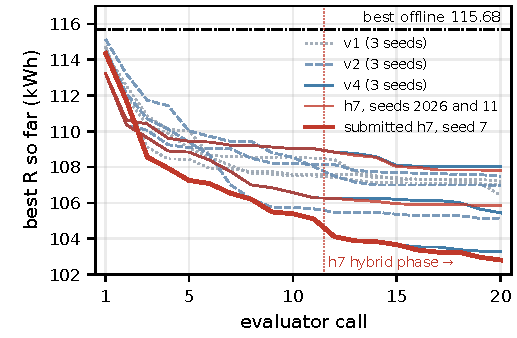
\includegraphics[width=\columnwidth]{figures/convergence.pdf}
\caption{每次调用后的平均最佳实测 $R$；阴影：种子间的范围。所有数值均为仿真器实测值。}
\label{fig:convergence}
\end{figure}

\textbf{RQ1：分块结构是否有效？} 去掉分块结构及两条依赖它的规则、其余不变，平均最终 $R$ 从 106.19 升到 107.84（$+1.65$~kWh，
$p=0.078$，各六个种子），并且平均而言 v4j 从第二次调用起就落后于 v4（第 10 次调用后的均值：108.48 对 107.12；
图~\ref{fig:convergence}）。单看这一差异，它没有达到 5\,\% 的显著性水平。v2 同样没有平台过滤和坐标重新施加，因此它把分块和
这两条规则分开了，但没有和后验份额、不重复规则以及第 1 次调用的八个跳跃点（从未命中）分开；v2 同样优于 v4j（$-1.37$~kWh，$p=0.041$）。在各分块下降变体之间，偏移偏置和分配都没有
可测地改变最终 $R$（两两比较 $p\ge0.48$），因此我们也把全部 15 次分块下降运行合起来与 v4j 比较：v4j 高 $+1.40$~kWh，$p=0.024$。
这两个比较都是在主比较之后选定的，所以我们把它们视为佐证，而不是证明。在这 15 次运行内部
可以看到这一机制。仅组合这一步（即每个新基点在尝试任何新移动之前相对上一个最好点的增益）就贡献了总下降的 33.0\,\%。组合点
有 83.7\,\% 低于当前最好点，加性预测~\eqref{eq:add} 的误差中位数为 $0.000$、平均绝对误差为 0.17~kWh（59\,\% 在 0.1 以内）；而
代理模型挑选的点平均比预测高 3.54~kWh（平均绝对误差 4.89），命中率为 4.2\,\%。在 43\,\% 的调用中，有两栋或以上的建筑在同一
批次中改进，因此组合不只是可用，而且确实被用上了。去掉分块后，代理模型挑选的点偏差更大（平均绝对误差 7.08），因为联合
移动离数据更远。

\begin{figure}[t]
\centering
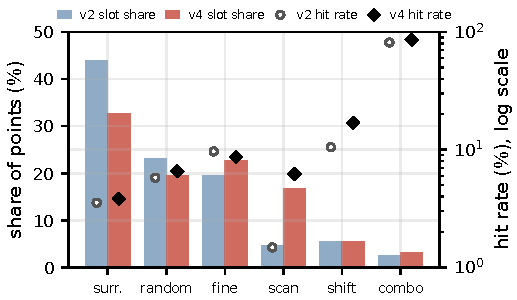
\includegraphics[width=\columnwidth]{figures/allocation.pdf}
\caption{各移动类别的点数份额（柱）与命中率（标记），汇总 v2 和 v4 的所有种子。命中指单块点低于其调用的基点，或基点与组合点（``combo''）低于上一个最好点。}
\label{fig:alloc}
\end{figure}

\textbf{RQ2：证据驱动的分配是否有效？} 没有可测的效果。在各六个种子上，v4 和 v2 分别停在 106.19 和 106.47（$-0.28$~kWh，
$p=0.76$）。平均而言 v4 在每一次调用都领先，但最多只领先 0.74~kWh（第 3 次调用），远在种子间的波动范围之内。这些规则确实做到了
设计要做的事（图~\ref{fig:alloc}）：后验份额把 11 个百分点的名额从代理模型挑选移走（44.0\,\% $\to$ 32.6\,\%；v4 中命中率为
3.8\,\%），转给扫描（4.6\,\% $\to$ 16.7\,\%）；扫描一旦跨出检测到的平台，命中率就从 1.5\,\% 升到 6.2\,\%。然而多出来的命中都很小：
扫描只贡献了 v4 下降量的 7.0\,\%，后期（第 11--20 次调用）从不同的权重向量返回本次运行已测过的 $R$ 的点所占比例仍在 31\,\% 左右（v2 为 32.6\,\%，
v4 为 31.3\,\%）。最初三个种子曾显示 0.93~kWh 的增益，另外三个种子使它消失了。

\textbf{其他变体与提交的策略。} 两次避免过早给每栋建筑锁定一种主导目标组合的尝试（顶点探测和并行通道），以及一个超参数
固定的代理模型，都没有超过 v4（三个种子上的均值分别为 106.26、106.86 和 106.22，v4 为 106.19）。一个独立的整批贝叶斯优化（加性 GP，每次
调用 24,000 个候选）在其唯一一次运行中达到 105.99，与 v4 的均值持平。提交的 h7 用提交的种子达到 102.81；它在自己的三个种子上的
第 1--11 次调用都与 v4 完全相同，因此在这三个种子上可以与 v4 配对，配对平均差为 $-0.09$（$-0.47$、$-0.24$、$+0.43$），即与 v4 无法区分。

\textbf{可复现性。} 从日志重新计算提交的运行，全部 20 个批次完全一致（最大 $|\Delta W|=0$）。在第二台机器上用评分运行包
跑另外两个种子，重放了第 1--11 次调用这 1,100 个点（2 个种子 $\times$ 11 次调用 $\times$ 50 个点）的 $R$：与对应的 v4 预演（用另一套框架、在另一台机器上运行）完全相同（只有
四个权重向量的最后一位不同，以及两个平局的候选交换了位置）。
